% Gallery figure source
% Summary: Rooted phylogenetic networks are usually interpreted as directed acyclic graphs. Reticulation can create a cycle in the underlying undirected graph, but arrows still follow a consistent older-to-younger time order.
\documentclass[tikz,border=6pt]{standalone}
% Shared color palette
\usepackage[T1]{fontenc}
\usepackage[utf8]{inputenc}
\usepackage{lmodern}
\usepackage{microtype}
\usepackage{amsmath,amssymb,mathtools}
\usepackage{xcolor}
\usepackage{tikz}
\usetikzlibrary{arrows.meta,positioning,calc,fit,backgrounds,decorations.pathreplacing,shapes.geometric,shadows.blur}

\definecolor{mainblue}{RGB}{42,85,132}
\definecolor{deepgreen}{RGB}{30,105,70}
\definecolor{burntorange}{RGB}{190,90,25}
\definecolor{softgray}{RGB}{245,246,248}
\definecolor{darkgray}{RGB}{70,70,70}
\definecolor{violet}{RGB}{110,70,150}

\newcommand{\given}{\,|\,}
\newcommand{\Ne}{N_{e}}
\newcommand{\ARG}{\mathrm{ARG}}
\newcommand{\MRCA}{\mathrm{MRCA}}
\newcommand{\GMRCA}{\mathrm{GMRCA}}

% Shared TikZ styles
\tikzset{
  tip/.style={circle,fill=black,inner sep=1.6pt},
  nodept/.style={circle,fill=black,inner sep=1.4pt},
  sampled/.style={rectangle,fill=black,inner sep=2.2pt},
  branch/.style={line width=0.8pt},
  retic/.style={circle,draw=burntorange,fill=burntorange!25,line width=0.8pt,inner sep=2.0pt},
  event/.style={circle,draw=mainblue,fill=mainblue!15,line width=0.8pt,inner sep=1.8pt},
  arr/.style={-{Latex[length=2.0mm]},line width=0.8pt},
  faint/.style={line width=0.7pt,draw=gray!55},
  parentedge/.style={-{Latex[length=2.0mm]},line width=0.9pt,draw=burntorange},
  treeedge/.style={-{Latex[length=2.0mm]},line width=0.9pt,draw=black},
  segment/.style={line width=4pt,line cap=round},
  dashedretic/.style={-{Latex[length=2.0mm]},line width=0.9pt,draw=burntorange,dashed}
}


\begin{document}
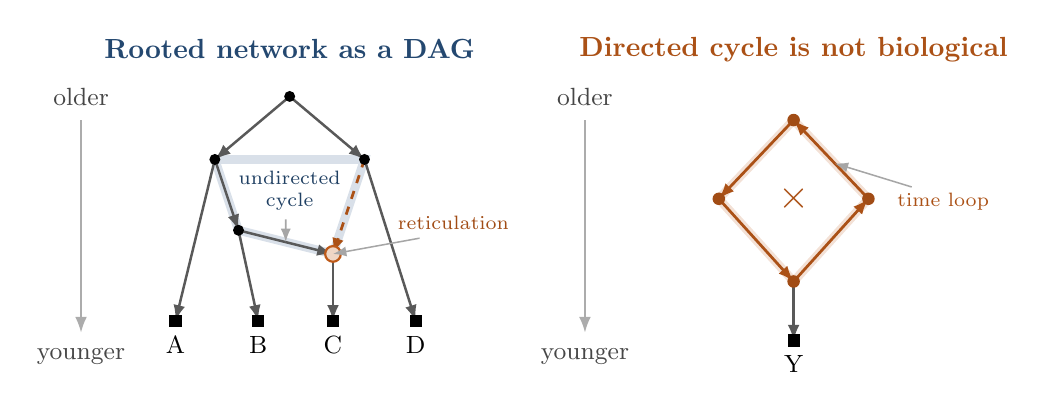
\begin{tikzpicture}[
  scale=1.0,
  timeedge/.style={-{Latex[length=2.0mm]},line width=.9pt,draw=darkgray!90},
  reticedge/.style={-{Latex[length=2.0mm]},line width=1.0pt,dashed,draw=burntorange!90!black},
  cycleedge/.style={line width=3.2pt,draw=mainblue!18,line cap=round},
  badedge/.style={-{Latex[length=2.0mm]},line width=1.0pt,draw=burntorange!90!black},
  badcycle/.style={line width=3.2pt,draw=burntorange!18,line cap=round},
  tiplabel/.style={font=\small},
  paneltitle/.style={font=\bfseries},
  note/.style={font=\small,align=center,text width=5.3cm,text=darkgray},
  callout/.style={font=\scriptsize,align=center,text=darkgray},
  callarr/.style={-{Latex[length=1.7mm]},line width=.55pt,draw=gray!70}
]

\begin{scope}
  \node[paneltitle,text=mainblue!85!black] at (2.2,4.15)
    {Rooted network as a DAG};

  \node[font=\small,text=darkgray] at (-0.45,3.55) {older};
  \node[font=\small,text=darkgray] at (-0.45,0.25) {younger};
  \draw[-{Latex[length=2mm]},draw=gray!65,line width=.7pt] (-0.45,3.25)--(-0.45,0.55);

  \coordinate (r)  at (2.2,3.55);
  \coordinate (u)  at (1.25,2.75);
  \coordinate (v)  at (3.15,2.75);
  \coordinate (w)  at (1.55,1.85);
  \coordinate (h)  at (2.75,1.55);
  \coordinate (A)  at (0.75,0.70);
  \coordinate (B)  at (1.80,0.70);
  \coordinate (C)  at (2.75,0.70);
  \coordinate (D)  at (3.80,0.70);

  \draw[cycleedge] (u)--(v)--(h)--(w)--(u);

  \draw[timeedge] (r)--(u);
  \draw[timeedge] (r)--(v);
  \draw[timeedge] (u)--(A);
  \draw[timeedge] (u)--(w);
  \draw[timeedge] (w)--(B);
  \draw[timeedge] (w)--(h);
  \draw[timeedge] (v)--(D);
  \draw[reticedge] (v)--(h);
  \draw[timeedge] (h)--(C);

  \foreach \p in {r,u,v,w}{
    \node[nodept] at (\p) {};
  }
  \node[retic] at (h) {};

  \foreach \p/\lab in {A/A,B/B,C/C,D/D}{
    \node[sampled] at (\p) {};
    \node[below=2pt,tiplabel] at (\p) {\lab};
  }

  \node[callout,text=mainblue!75!black] at (2.20,2.35)
    {undirected\\ cycle};
  \draw[callarr] (2.15,1.99)--($(w)!0.5!(h)$);

  \node[callout,text=burntorange!85!black] at (4.28,1.95)
    {reticulation};
  \draw[callarr] (3.85,1.75)--(h);
\end{scope}

\begin{scope}[xshift=6.4cm]
  \node[paneltitle,text=burntorange!90!black] at (2.2,4.15)
    {Directed cycle is not biological};

  \node[font=\small,text=darkgray] at (-0.45,3.55) {older};
  \node[font=\small,text=darkgray] at (-0.45,0.25) {younger};
  \draw[-{Latex[length=2mm]},draw=gray!65,line width=.7pt] (-0.45,3.25)--(-0.45,0.55);

  \coordinate (x1) at (2.2,3.25);
  \coordinate (x2) at (1.25,2.25);
  \coordinate (x3) at (3.15,2.25);
  \coordinate (x4) at (2.2,1.20);
  \coordinate (Y)  at (2.2,0.45);

  \draw[badcycle] (x1)--(x2)--(x4)--(x3)--(x1);

  \draw[badedge] (x1)--(x2);
  \draw[badedge] (x2)--(x4);
  \draw[badedge] (x4)--(x3);
  \draw[badedge] (x3)--(x1);
  \draw[timeedge] (x4)--(Y);

  \foreach \p in {x1,x2,x3,x4}{
    \node[circle,fill=burntorange!85!black,inner sep=1.6pt] at (\p) {};
  }
  \node[sampled] at (Y) {};
  \node[below=2pt,tiplabel] at (Y) {Y};

  \node[font=\Large,text=burntorange!90!black] at (2.2,2.25) {$\times$};

  \node[callout,text=burntorange!90!black] at (4.10,2.22)
    {time loop};
  \draw[callarr] (3.70,2.40)--($(x3)!0.45!(x1)$);
\end{scope}

\end{tikzpicture}
\end{document}
